% !TEX root = ../thesis.tex

\chapter{Grundlagen}
\label{ch:grundlagen}

Zum Verständnis des Themas der Arbeit ist die Erklärung einiger Grundlagen notwendig.
In \ref{sec:3d-bilder} und \ref{sec:meshrepr} werden zunächst einmal wichtige Grundbegriffe und Datenstrukturen erläutert, die bei der Arbeit mit 3D-Daten auftreten.
Anschließend werden die verwendeten Bibliotheken \ac{PCL} und \ac{ROS} erklärt, welche zur Datenverarbeitung bzw. zur Robotersteuerung verwendet wurden.
%TODO Mikado-API / -Elemente in den Grundlagen beschreiben  # Eher in Vorhandene Arbeit...
Außerdem sind selbstverständlich die bereits bestehenden Elemente des Mikado-Projekts relevant, da diese Arbeit fundamental darauf aufbaut.


\section{Aufnahme und Speicherung von 3D-Bildern}
\label{sec:3d-bilder}

%TODO Tiefergehende / fundiertere Informationen zur Aufnahme. Quellen fehlen.
Zur Aufnahme von 3D-Bilddaten gibt es mehrere verschiedene Möglichkeiten.
Ein LIDAR-System sendet beispielsweise mehrere Lichtstrahlen in verschiedene Richtungen, die anschließend Informationen über die Entfernung zu einem Objekt in diesem Punkt liefern.
Eine Stereokamera liefert im Gegensatz dazu zwei Bilder, die anschließend durch spezielle Software zu einem dreidimensionalen Bild zusammengesetzt werden.
Eine weitere Möglichkeit besteht darin, ein bestimmtes Muster auf die Umgebung zu projezieren, dieses dann aus einer anderen Perspektive aufzunehmen und aus der räumlichen Verzerrung des Musters die Tiefe zu errechnen.

Die so gewonnenen Informationen lassen sich durch mehrere verschiedene Datenmodelle repräsentieren.


\subsection{Tiefenbild}
\label{subsec:tiefenbild}

Ein Tiefenbild ist eine einfache Möglichkeit, in einem zweidimensionalen Bild zusätzlich Informationen über die Entfernung der Kamera zu Objekten abzuspeichern.
Diese Technik ist unter Anderem aus der Computergrafik bekannt, wo sie beim Z-Buffering Anwendung findet \cite{strasser1974schnelle}.
Dabei werden sowohl das aufgenommene Bild, aber zusätzlich auch ein 2D-Array mit der Tiefeninformation des zugehörigen Pixels gespeichert.

So kann das originale 2D-Bild um eine dritte Dimension erweitert werden, wodurch sich beispielsweise dreidimensionale Formen modellieren oder rekonstruieren lassen \cite{arsalan2017synthesizing}.
Auch in der 3D-Fotografie finden Tiefenbilder Anwendung \cite{redert2006philips}.

\begin{figure}[ht]
	\centering
	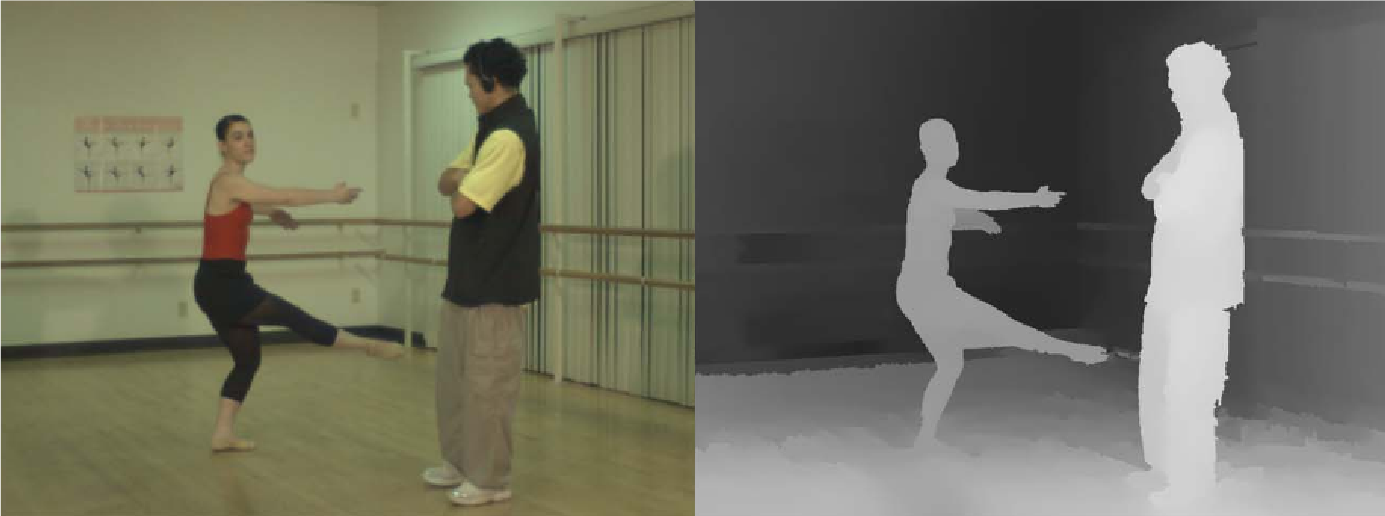
\includegraphics[width=0.66\textwidth]{images/depth_map.png}
	\caption{Depth Map eines 2D-Farbbilds. Entnommen aus \cite[S.649]{muller2010depth}}
	\label{fig:depth_map}
\end{figure}

Tiefenbilder haben im Vergleich zu anderen möglichen Datenmodellen den Vorteil, dass 2D-Bilder sehr einfach um zugehörige Tiefeninformationen erweitert werden können.
Jedoch gibt es auch einige Nachteile, die nicht umgangen werden können:

\begin{itemize}
\item Die 3D-Daten sind ausschließlich aus der Kameraperspektive vorhanden.
Um Informationen aus einer anderen Perspektive zu erhalten, muss erst aufwändig umgerechnet werden.
\item Da (in den meisten Fällen) nur ein zweidimensionales Array für die Tiefeninformation angelegt wird, können nur die Entfernungen zu den der Kamera nächsten Objekte gespeichert werden.
Verdeckte, reflektierende oder durchsichtige Oberflächen können nicht gespeichert werden.
\item Das Array ist an die Auflösung der Kamera gebunden.
Insbesondere bei großer Entfernung zu Objekten werden diese aufgrund des Bildwinkels sehr schlecht abgetastet, was später zu Aliasing-Effekten führen kann.
\item Die Bittiefe der Werte im Array kann - je nach gewünschter Auflösung - zu niedrig sein, bzw. muss erhöht werden.
Eine typische Farbtiefe eines Grauwertbilds von 8 Bit repräsentiert beispielsweise nur $2^8 = 256$ Stufen - was schnell zu wenig wird.
Insbesondere bei hoher notwendiger Auflösung im nahen Bereich, aber gleichzeitig vorhandenen weit entfernten Objekten kann dies zum Problem werden.
\end{itemize}


\subsection{Voxel Grid}
\label{subsec:voxel-grid}

Bei einem als Bitmap vorliegendes 2D-Bild werden die Bilddaten diskretisiert in einem zweidimensionalen Array $I$ gespeichert.
Mit einer Bittiefe $b$, einer Bildhöhe $i$ und einer Bildbreite $j$ ergibt sich damit folgende Matrix:

$$I = \begin{pmatrix}
v_{11} & v_{12} & v_{13} & \cdots\\
v_{21} & v_{22} & v_{23} & \cdots\\
v_{31} & v_{32} & v_{33} & \cdots\\
\vdots & \vdots & \vdots & \ddots
\end{pmatrix}, v_{ij} \in [0; 2^b) \wedge b, i, j \in \mathbb{N}^+$$

Dieses Prinzip lässt sich einfach auf den dreidimensionalen Raum erweitern.
Die so erhaltene Datenstruktur nennt sich Voxel Grid.
Als Voxel bezeichnet man somit eine einzelne Datenzelle im 3D-Array, also das dreidimensionale Äquivalent zum Pixel.

Voxel Grids finden in vielen Bereichen Anwendung, zum Beispiel in der Medizin. %TODO CITATION
Auch zum Downsampling von Punktwolken werden sie verwendet \cite{pclVoxelGrid}. %TODO Zu Punktwolken / Implementierung...

Gegenüber einem Tiefenbild hat ein Voxel Grid den inhärenten Nachteil, dass Speicherplatz für jeden Voxel benötigt wird.
Dies führt schnell zu großem Speicherbedarf $M$, da dieser kubisch zur Auflösung $r$ steigt: $M = r_x * r_y * r_z * b$ bei Bittiefe $b$.

Ein Vorteil im Vergleich zum Tiefenbild ist jedoch, dass die Abhängigkeit von der Kameraperspektive wegfällt.
Dadurch können hier auch Objekte modelliert werden, die im Tiefenbild durch eine Verdeckung versteckt wären.

Desweiteren ist der Raum einheitlich diskretisiert.
Dies kann je nach Szene und Kameraposition sowohl ein Vor- als auch ein Nachteil sein:
Bei einem Tiefenbild nimmt der Abstand der Messpunkte mit der Tiefe ab.
Ist die Entfernung zwischen Objekt und Kamera gering, werden diese mit einer deutlich besseren Auflösung abgetastet als sehr weit entfernte Objekte.
Im Voxel Grid werden Objekte jedoch überall gleich abgetastet.
Dies führt zu verbesserter Auflösung bei entfernten und zu schlechterer Auflösung bei nahen Objekten.


\subsection{Punktwolken}
\label{subsec:punktwolken}

Ein weiteres häufig verwendetes Datenmodell ist eine Punktwolke.
Als Punktwolke bezeichnet man eine Menge $M \subset \mathbb{R}^3$ von Punkten im (mindestens) dreidimensionalen Raum.
Zusätzlich zur räumlichen Information können auch noch weitere Daten pro Punkt gespeichert sein, wie RGB-Werte, Genauigkeit oder Objektklasse (falls schon eine Segmentierung vorgenommen wurde).
Dadurch gilt:
$$M = \begin{pmatrix}
p_x^1 & p_y^1 & p_z^1 & \cdots\\
p_x^2 & p_y^2 & p_z^2 & \cdots\\
p_x^3 & p_y^3 & p_z^3 & \cdots\\
\vdots & \vdots & \vdots & \ddots
\end{pmatrix}$$

\begin{figure}[ht]
	\centering
	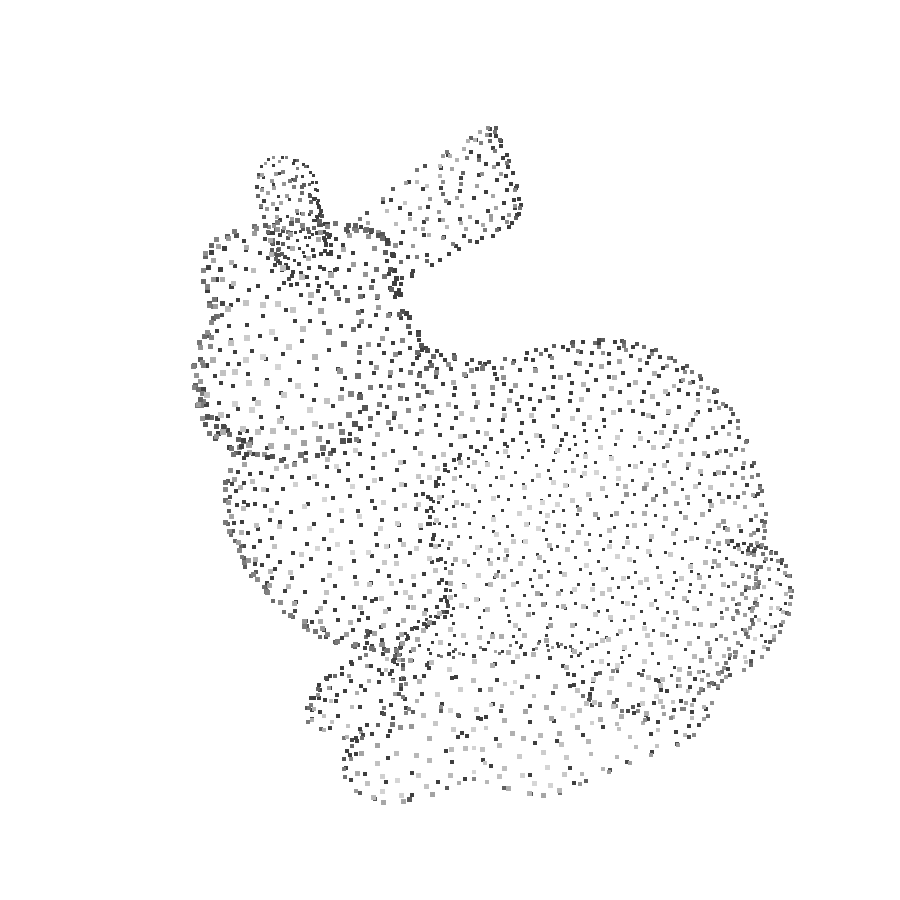
\includegraphics[width=0.66\textwidth, frame]{images/bunny_pcd.png}
	\caption{Punktwolke des Stanford Bunny \cite{stanfordbunny}}
	\label{fig:bunny_pcd}
\end{figure}

Die Nutzung von Punktwolken bringt im Vergleich zu anderen 3D-Datenmodellen einige Vorteile.

\begin{itemize}
\item Die zugrundeliegende Datenstruktur ist extrem trivial; es handelt sich um eine einfache Liste.
Dies ermöglicht sehr schnelle Operationen, wie zum Beispiel das Hinzufügen eines Punktes.
Es lässt sich sehr einfach über die Punkte iterieren.
\item Der Speicherbedarf einer Punktwolke wächst dynamisch, und zwar linear mit der Zahl der enthaltenen Punkte.
Beim Voxel Grid muss dagegen bereits am Anfang Speicher für jede Zelle reserviert werden, egal ob ein Punkt enthalten ist oder nicht.
\item Man ist nicht, wie beim Tiefenbild oder Voxelgrid, auf eine feste Anzahl an Punkten limitiert.
Beim Tiefenbild können maximal $n * m$ Punkte (ein Wert pro Pixel) mit einer Tiefeninformation versehen werden, beim Voxel Grid maximal $x * y * z$ Punkte (ein Wert pro Voxel).
Eine Kapazitätserweiterung, wie beispielsweise das Hinzufügen neuer Pixelspalten oder -zeilen im Tiefenbild, entfallen bei der Punktwolke.
\item Die Auflösung ist nur durch die Gleitkommagenauigkeit der Maschine limitiert.
Beim Voxel Grid ist sie im Gegensatz dazu durch die Größe der Voxel limitiert.
Beim Tiefenbild ist die Auflösung abhängig von der Tiefe im Bild - bei weiter entfernten Objekten ist die Auflösung auch niedriger.
\end{itemize}

Es gibt jedoch auch einige Nachteile gegenüber den anderen Repräsentationen:

\begin{itemize}
\item Die Rekonstruktion eines Meshs ist nicht eindeutig.
Beim Voxel Grid lässt sich, beispielsweise mithilfe des Marching-Cubes-Algorithmus \cite{lorensen1987marching}, ein eindeutiges Mesh rekonstruieren.
Bei einer Punktwolke ist im Gegensatz dazu nicht festgelegt, welche Punkte miteinander verbunden werden sollen.
\item Viele Techniken aus der Bildverarbeitung (wie zum Beispiel Segmentierung, Filterung usw.) lassen sich auf Tiefenbilder direkt übertragen.
Dies ist bei Punktwolken nicht möglich.
\end{itemize}


\section{Meshrepräsentationen}
\label{sec:meshrepr}

\begin{figure}[ht]
	\centering
	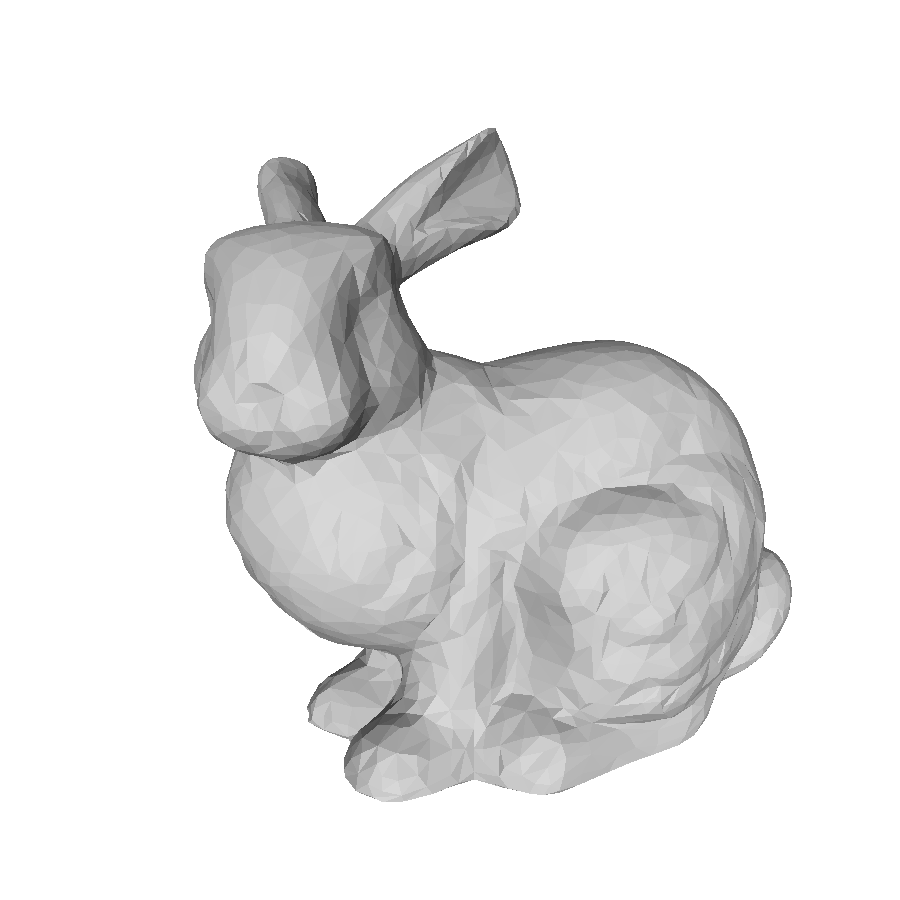
\includegraphics[width=0.66\textwidth, frame]{images/bunny_mesh.png}
	\caption{Mesh des Stanford Bunny \cite{stanfordbunny}}
	\label{fig:bunny_mesh}
\end{figure}


\section{Point Cloud Library}
\label{sec:pcl}


\section{Robot Operating System}
\label{sec:ros}
